\section{Motivation}

% AI

In the last decades, the advances in computers architecture and computer science have pushed the research frontier to produce super intelligent algorithms, capable of dealing with difficult classification problems of subtle and inherently human concepts, or even hard decision making tasks in challenging situations. We can see intelligent algorithms applied to speech and image recognition, email spam classification, advertising, fraud detection, autonomous self-driving cars, virtual assistants, security, finance and several other applications in our lives \cite{AIapplications}. Never in history we have witnessed such a great bet in the future of machines.

% cutting edge achievments

Besides, most recently, the cutting edge achievements in AI have shown algorithms capable of overcoming top human intelligence in difficult problems. In 2015, Google DeepMind created an AI that learned how to play 49 Atari games using the same learning algorithm (including the same hyper parameters), using as the input only the pixels from the screen. The algorithm, called Deep Q-Learning \cite{RLNature2015}, was a breakthrough achievement in the mission of accomplishing a general purpose machine learning agent in a wide variety of games.

In the same year, DeepMind left another big mark in the human history. A computer program called AlphaGo defeated Lee Sedol, the best human Go player, for the first time. Go consists of a very complex board game, with more than $10^{170}$ configurations, and represents one of the biggest challenges to human intelligence and an unconceivable problem to a computer until then. Going even further, in 2017, \cite{AlphaGoZero} introduced AlphaGo Zero, an evolution of the previous version, capable of leaning how to play without any outside data from human games, but just playing with itself. Figure \ref{fig:deepmind_examples} illustrates these successful examples.

\begin{figure}[ht]
  	\centering
  	\begin{subfigure}[b]{0.9\textwidth}
              \centering
	 		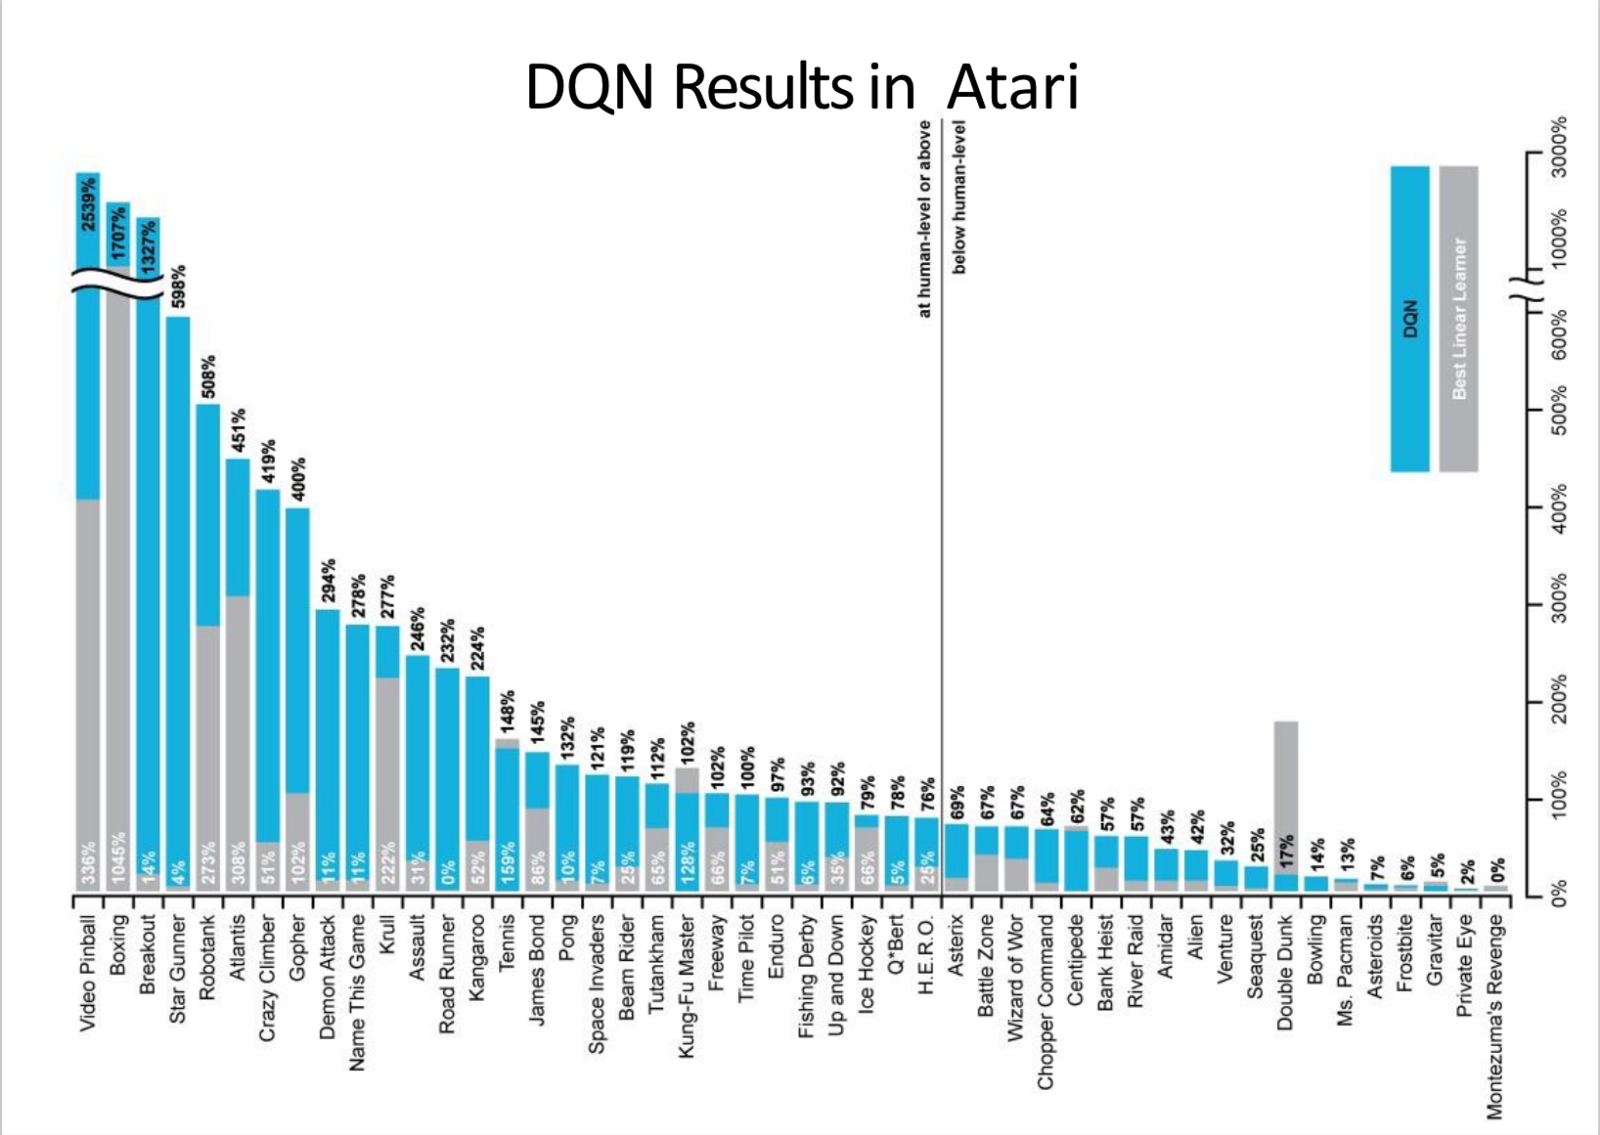
\includegraphics[height=0.35\textheight]{Chapter1/DQN-atari.png}	
	 		\caption{DQN results in Atari games}
     \end{subfigure}
     
	 \begin{subfigure}[b]{0.45\textwidth}
              \centering
	 		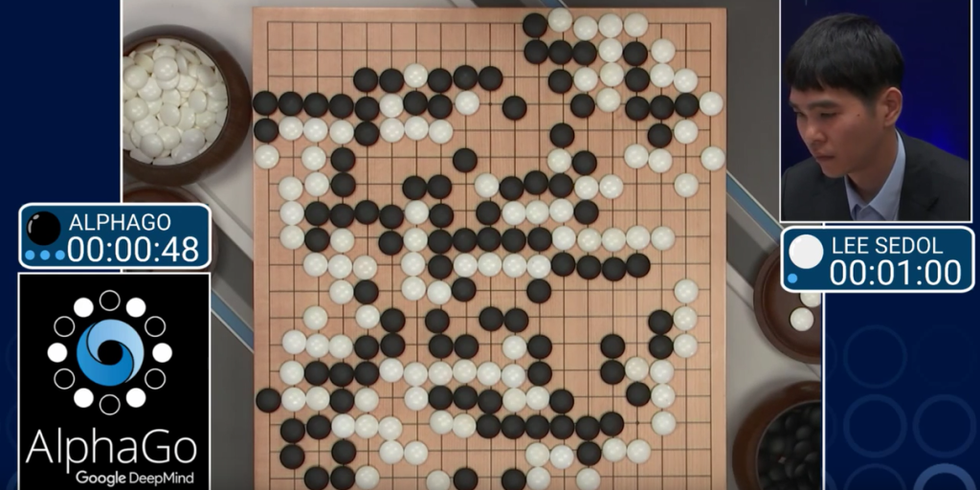
\includegraphics[height=0.2\textheight]{Chapter1/alphago.png}
	 		\caption{AlphaGo against Lee Sedol}
	 \end{subfigure}
	 ~~
      \begin{subfigure}[b]{0.45\textwidth}
              \centering
	  	    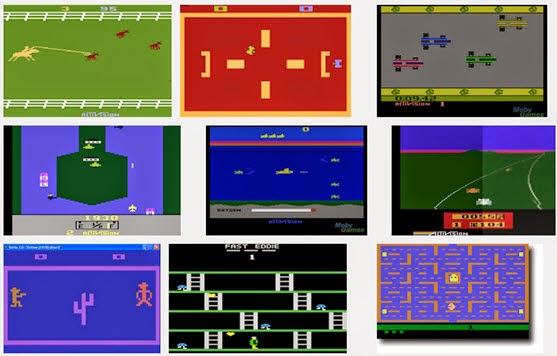
\includegraphics[height=0.2\textheight]{Chapter1/atari.jpg}
	  	    \caption{Different Atari games}
	 \end{subfigure}
	     
	 \caption{DeepMind recent achievements.}
	\label{fig:deepmind_examples}
\end{figure}

% robotics

%Another big field in Computer Science which has been receiving great attention of the research community is mobile robotics. Robotics can address state of the art challenges in different domains, such as Electronics Engineering, Mechanical Engineering, Control Theory and, of course, Machine Learning.

Another big field in Computer Science is mobile robotics, which plays a big role in the future of the industry and part of the forefront of academic research recently. Robotics can address state of the art challenges in different domains, such as Electronics Engineering, Mechanical Engineering, Control Theory and, of course, Machine Learning.

AI finds in Robotics several applications, as computer vision, path planning and even motion control, and in this last one we can find one of its biggest challenges. In Atari and board games we can easily define a goal, win, but how can we define the agility and flexibility of a walk or a jump movement? In this sense, several works have been conducted in the problem of trying to reproduce human movements in humanoid robotics agents, and more specifically, in a simulated scenario.

\begin{figure}[ht]
  	\centering
  	\begin{subfigure}[b]{0.45\textwidth}
              \centering
	 		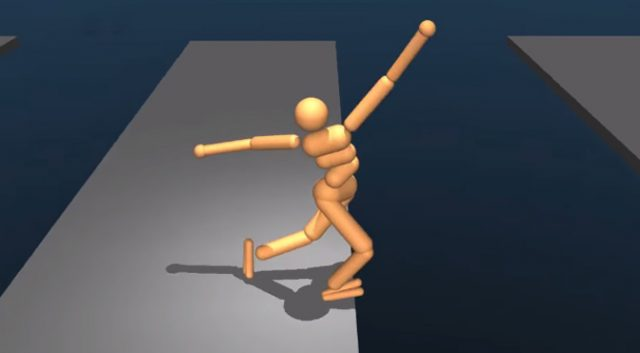
\includegraphics[height=0.13\textheight]{Chapter1/humanoid-deepmind1.jpg}	
     \end{subfigure}
     
	 \begin{subfigure}[b]{0.45\textwidth}
              \centering
	 		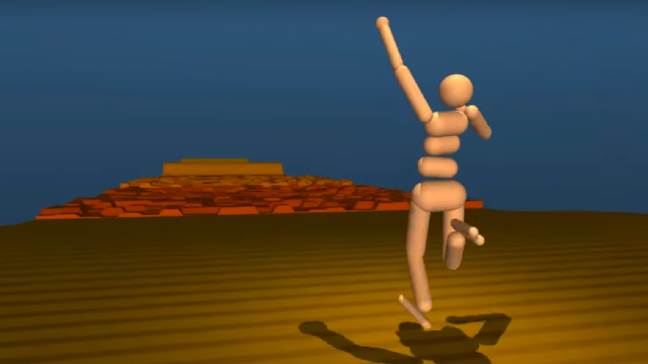
\includegraphics[height=0.13\textheight]{Chapter1/humanoid-deepmind2.png}
	 \end{subfigure}
	 ~~
      \begin{subfigure}[b]{0.45\textwidth}
              \centering
	  	    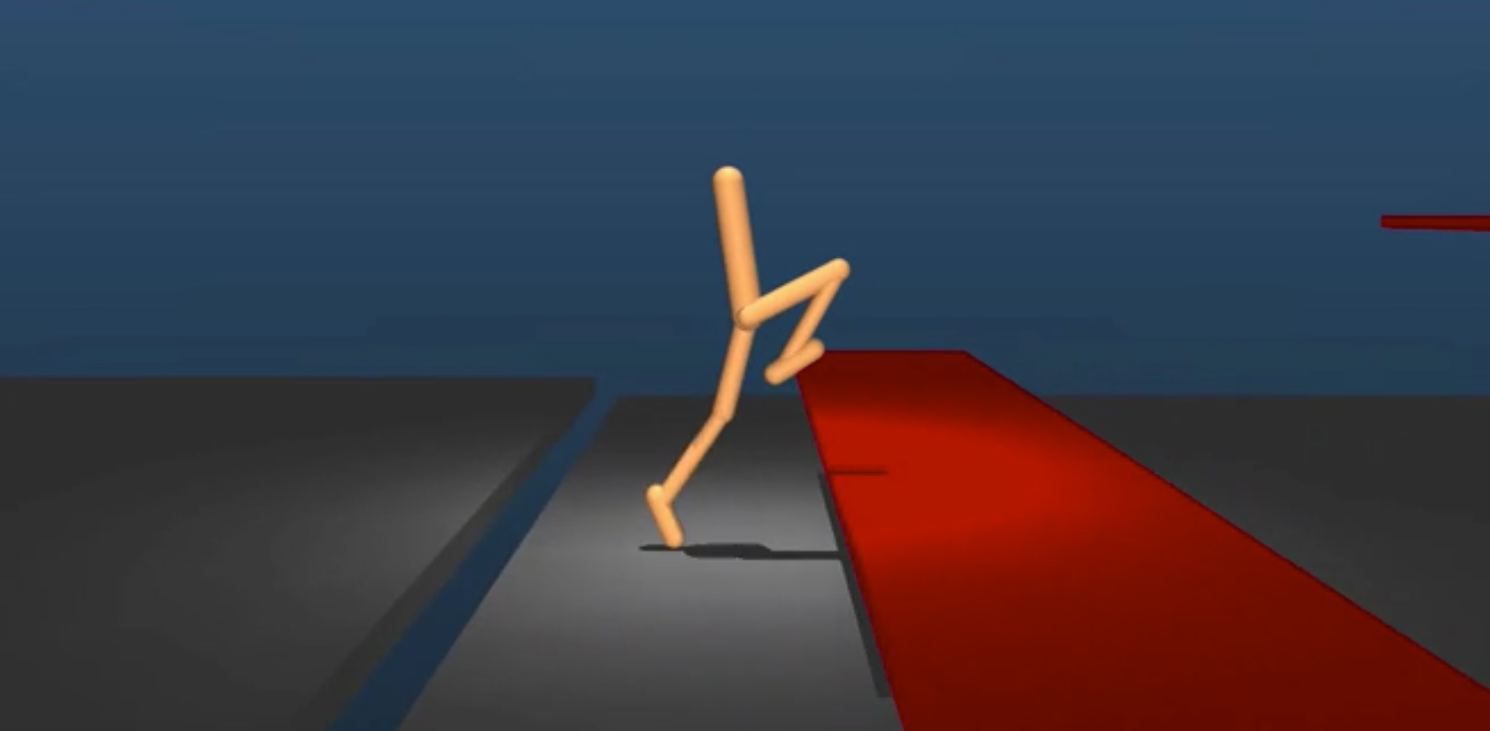
\includegraphics[height=0.13\textheight]{Chapter1/humanoid-deepmind3.png}
	 \end{subfigure}
	     
	 \caption{Simulated humanoid agent movements and AI.}
	\label{fig:humanoid_AI}
\end{figure}

% robocup

One of the biggest initiatives of the research community to foster the study of robotics is RoboCup. RoboCup established itself as one of the main international robotics competition in the world, and also organizes a scientific conference to share the latest works in the field. It pushes state-of-the-art research in robotics by maintaining different technical challenges, among them the most famous are making robots play soccer, with the mission of developing a humanoid robot team capable of winning the champion of FIFA World Cup in 2050.

One RoboCup's particular league is the RoboCup 3D Soccer Simulation League, consisting of a soccer match between two teams, each one composed by up to 11 simulated NAO robots from Aldebaran Robotics. This league addresses both high level and low level robotics challenges, like path planning and locomotion, and greatly helped improving our understanding of human movements like walking and kicking the ball.

\begin{figure}[ht]
  	\centering
  	\begin{subfigure}[b]{0.45\textwidth}
              \centering
	 		
\includegraphics[height=0.13\textheight]{Chapter1/RoboCup.png}	
     \end{subfigure}
     
	 \begin{subfigure}[b]{0.45\textwidth}
              \centering
	 		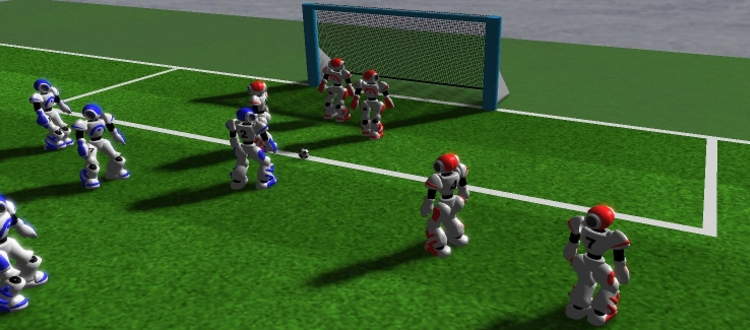
\includegraphics[height=0.13\textheight]{Chapter1/SS3D.png}
	 \end{subfigure}
	     
	 \caption{Robocup symbol and Soccer 3D Simulation league match.}
	\label{fig:robocup}
\end{figure}

\section{Problem Statement}

Inspired by the RoboCup 3D Soccer Simulation (Soccer3D or SS3D) league, this dissertation's objective is to learn a low level soccer behavior for simulated humanoid robots, more specifically, the behavior of kicking the ball towards a planned final distance from the agent. In this sense, the algorithm should input the current agent state, including its joints positions and distance to the ball, and output sequential controls for each robot's joint.

\section{Approach}

Instead of employing a deterministic and off-line built single movement, called Keyframe movement, we intend to use a model-free deep reinforcement learning based approach that tries to learn the desired behavior by interacting with an environment (the simulation server) and receiving rewards depending on which actions it chooses.
The chosen strategy for this will be first learning a behavior that imitates the current kick movement, as described in the work \cite{deepmimic}, and then improving this behavior by reinforcement learning, targeting the desired position given as an input to the policy function.
% PERGUNTAR MELHOR PRO MANGA

\section{Literature Review}

Reinforcement Learning techniques have been in increasingly study in the past 30 years. In this time, some specific works have established  famous breakthroughs in this field. For instance, Temporal-Difference (TD) learning algorithms \cite{TDLearning} created the groundwork for many future RL algorithms, making use of value function estimation and policy and value iteration methods. In the same way, Q-Learning \cite{QLearning} introduced off-policy model-free learning with \textit{Sarsa}, estimating action-value functions and making room to future DRL algorithms.

After these works, \citen{REINFORCE} created a new paradigm presenting the REINFORCE algorithm, which introduces policy search methods. This technique estimates the optimal-policy function $\pi_*$ directly, without the need of value or action-value functions and works better in continuous action space, as we see in the robotics world. The most recent approaches developed make use and improve this method, such as the Deep Deterministic Policy Gradients (DDPG) algorithm, introduced by \cite{DDPG}, the Trust Region Policy Optimization (TRPO) algorithm, presented in \cite{TRPO}, and the Proximal Policy Optimization (PPO) algorithm, given in \cite{PPO}.

Another recent breakthrough in the RL field was given by Deep Neural Networks, making possible to escalate the classical algorithms to high dimensional problems. This process was marked by the incredible results of the Deep Q-Networks (DQN) algorithm \cite{RLNature2015}. This technique was able to learn 49 Atari games directly from raw pixels of the screen. It introduces the idea of modeling the action-value function by a neural network, and handles the inherently instability problem from value function approximation by introducing also two techniques: Experience Replay \cite{ReplayBuffer} and Target Networks \cite{RLNature2015}.

Meanwhile, some recent works started to address humanoid movements in the RL field. However, the main problem which comes with that endeavor is that simple rewards functions or naively selected ones, such as the score for the games problems, can lead to results that do not match the expectations. This is the common case in continuous control tasks, like locomotion. In this sense, \cite{deepmind1} proposed that rich and robust behaviors can emerge from simple reward functions, if the environment itself contains sufficient richness and diversity. This work introduces scenarios with a lot of obstacles and varying levels of difficulty, which are presented to the agent as an implicit curriculum, making possible to overcome increasingly hard challenges. A similar idea was also introduced by \cite{BengioCurrLearning}.

Other DeepMind's papers introduced methods to learn to imitate human movements, like \cite{deepmind2} and \cite{deepmind3}, which combines supervised learning and Generative Adversarial Imitation Learning (GAIL) \cite{gail}, in a way that accentuates their individual strengths and address their limitations.

Another recent state-of-the-art work in imitation learning is \cite{deepmimic}. This work makes it possible for a motion capture actor to supply a set of reference motions for style, and then generate goal-directed and physically realistic behaviors from them. The approach used for this is designing a reward function which combines rewarding motions that resemble reference animation data, and also achieving additional task objectives.

The most famous work that addresses the specific mission of kicking the ball towards a planned final distance from the agent in the Soccer3D environment is \cite{abbas}. In this work, the authors used a policy search approach to determine the optimal parameters for the kicking behavior policy $\pi(\theta | s)$, proposing the use of contextual relative entropy policy search with covariance matrix adaptation (CREPS-CMA) algorithm for this task.

However, we can see some limitations of this work that are possible to tackle. In \cite{abbas}, the authors still make use of a Keyframe based movement, and the policy $\pi(\theta | s)$ only outputs the initial and final frame position given the desired distance $s$. We propose a neural network based policy which inputs and outputs all the joints positions in run time, performing a closed loop behavior. Besides, there are more recent and cutting-edge RL algorithms that can be used to learn this task, such as DDPG, TRPO and PPO. Also, by making use of the approach described in \cite{deepmimic}, it is possible to overcome the initial challenge of learning a basic but complete behavior at first.

At last, we must cite the work \cite{TGMuzio}, which is one of the first works covering deep reinforcement learning and the SS3D, with similar tasks regarding humanoid locomotion. More specifically, this work handles the problem of developing a behavior for dribbling the ball against a single opponent, and provide successful solutions using DDPG, TRPO and PPO.

\section{Contributions}

This work's major contribution is applying recent deep reinforcement learning (DRL) algorithms in the task of learning a complete behavior to kick a ball towards a planned final distance from the agent in the Soccer3D environment domain. To the best of our knowledge, this work is the first that makes use of a DRL approach to develop a complete soccer behavior for this specific task.

\section{Outline of this Dissertation}

This dissertation is organized as follows:

\begin{itemize}
    \item \textbf{Chapter \ref{chap:introduction}} introduces this dissertation by describing the motivation 
    behind the problem we address, by the literature review and by summarizing the contributions.

    \item \textbf{Chapter \ref{chap:rl}} describes a brief theoretical background of reinforcement learning and neural networks.
    
    \item \textbf{Chapter \ref{chap:deep_rl}} describes a brief theoretical background of neural networks and some cutting-edge DRL algorithms

%    \item \textbf{Chapter \ref{chap:deep_learning}} constructs the building blocks of deep learning.

%    \item \textbf{Chapter \ref{chap:deep_rl}} provides the main deep reinforcement learning techniques used in our work.

%    \item \textbf{Chapter \ref{chap:methodology}} explains the methodology of this work, the tools that were used and how 
%    our environment was implemented.

%    \item \textbf{Chapter \ref{chap:contrib}} describes this dissertation's major contributions: 
%    how we formulated the learning tasks and how we modeled it to successfully
%    master them.

%    \item \textbf{Chapter \ref{chap:experiments}} evaluates our model in a few humanoid soccer tasks and describes our results.

%    \item \textbf{Chapter \ref{chap:conclusion}} concludes this dissertation and presents our ideas for future investigation.
\end{itemize}
